\subsection{Kødpopularitet}

Herunder er de mest gængse kødprodukter listet efter popularitet i følge En unavngiven kilde der følger miljøet tæt:\\
\begin{itemize}
\item Bacon \cite{bib:url:WikiBacon} - ingen introduktion nødvendig
\item Kylling (Chicken) \cite{bib:url:WikiChicken} - Kød fra små fjerklædte dinosaurnedstammende dyr.
\item Kalkun (Turkey) \cite{bib:url:WikiTurkey}- Kød fra lidt større fjerklædte dinosaurnedstammende dyr. De flyver vist ikke så godt længere og er derfor nemme at fange med en trefork
\item Svin (Pork) \cite{bib:url:WikiPork} - Kød der er en god bund i en fantastisk lagkage
\end{itemize}

\begin{center}
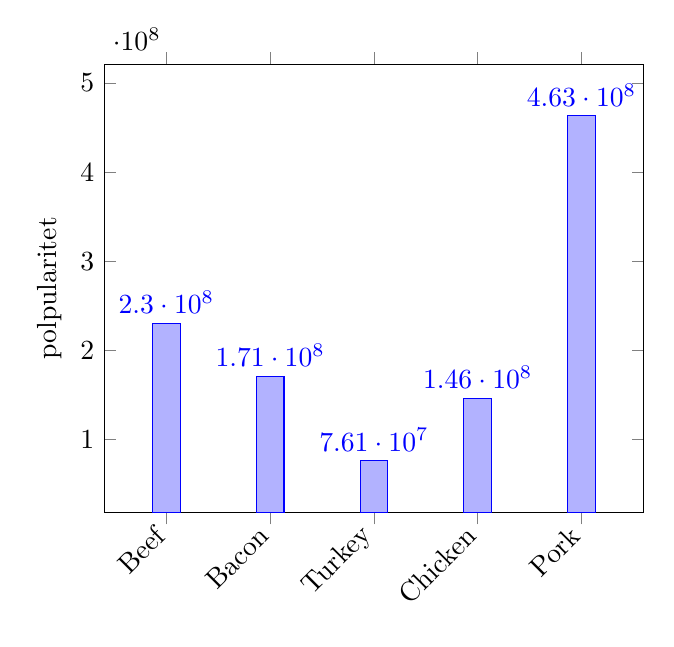
\begin{tikzpicture}
\begin{axis}[
ybar,
enlargelimits=0.15,
legend style={at={(0.5,-0.1)},
anchor=north,legend columns=-1},
ylabel={polpularitet},
symbolic x coords={Beef,	Bacon,	Turkey,	Chicken,	Pork},
xtick=data,
nodes near coords,
nodes near coords align={vertical},
x tick label style={rotate=45,anchor=east},
]
\addplot coordinates {(Beef,230000000) (Bacon,171000000) (Turkey,76100000) (Chicken,146000000) (Pork,463000000)};
\end{axis}
\end{tikzpicture}
\end{center}

En nærmere undersøgelse viser dog tydeligt Bacons position som svinets mest elskede kød:
\begin{itemize}
\item Bacon \cite{bib:url:WikiBacon}
\item Flæskesteg \cite{bib:url:WikiRoastPork}
\item Ham \cite{bib:url:WikiHam}
\item Loin \cite{bib:url:WikiLoin}
\item Spam\footnote{Well, there's egg and bacon; egg sausage and bacon; egg and spam; egg bacon and spam; egg bacon sausage and spam; spam bacon sausage and spam; spam egg spam spam bacon and spam; spam sausage spam spam bacon spam tomato and spam; spam spam spam egg and spam; spam spam spam spam spam spam baked beans spam spam spam or Lobster Thermidor a Crevette with a mornay sauce served in a Provencale manner with shallots and aubergines garnished with truffle pate, brandy and with a fried egg on top and spam.} \cite{bib:url:WikiSpam}
\item Spare Ribs \cite{bib:url:WikiSpareRibs}
\item Mørbrad \cite{bib:url:WikiTenderLoin}
\end{itemize}
\begin{center}
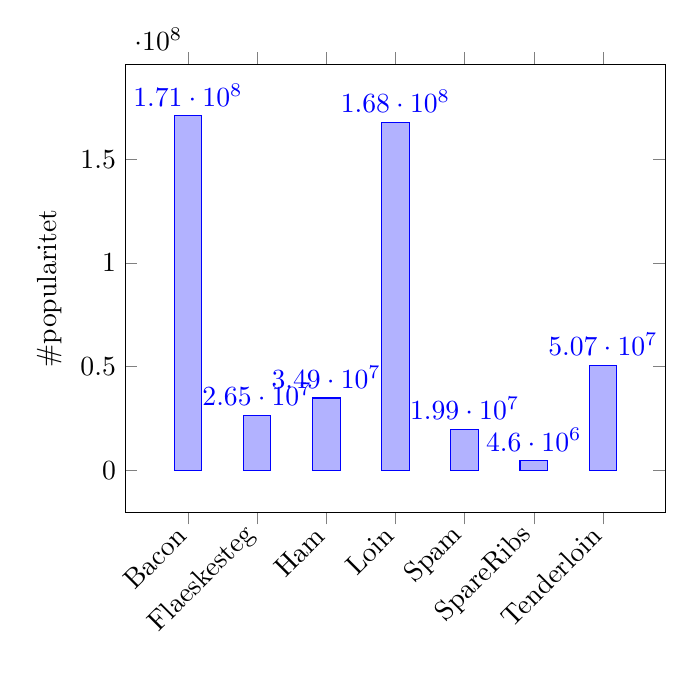
\begin{tikzpicture}
\begin{axis}[
ybar,
enlargelimits=0.15,
legend style={at={(0.5,-0.2)},
anchor=north,legend columns=-1},
ylabel={\#popularitet},
symbolic x coords={Bacon,Flaeskesteg,Ham,Loin,Spam,SpareRibs,Tenderloin},
xtick=data,
nodes near coords,
nodes near coords align={vertical},
x tick label style={rotate=45,anchor=east},
]
\addplot coordinates {(Bacon,171000000) (Flaeskesteg,26500000) (Ham,34900000) (Loin,168000000) (Spam,19900000)(SpareRibs,4600000)(Tenderloin,50700000)};
\end{axis}
\end{tikzpicture}
\end{center}

Heraf ses klart hvor populært bacon er; meget. Dette har medført en stigende tendens hvor mennesker er blevet navngivet efter dette fantastiske stykke kød:

\begin{itemize}
\item Kevin Bacon, skuespiller kendt for at være centrum for Hollywood \cite{bib:url:oracleofbacon}, \cite{bib:url:kevinBacon}, \cite{bib:url:wikikevinBacon}
\item Francis Bacon, Bagmanden bag den erkendelsesteori der nu kaldes empirisme, tidligere den baconske metode \cite{bib:url:wikifrancisBacon}, \cite{bib:url:wikiBaconisme}
\item Roger Bacon, Videnskabsmand der undervister som en af de første i brugen af videnskabelige metoder indenfor forskning \cite{bib:url:wikiRogerBacon}, \cite{bib:url:wikiRogerBaconMethod}
\item Bacon county - USA, opkaldt efter Augustus Bacon \cite{bib:url:wikiBaconCounty}, \cite{bib:url:wikiAugustusBacon}
\item Reginal Bacon, Britisk Admiral beundret for sine tekniske færdigeheder i planlægning og udkæmpelse af såslag. \cite{bib:url:wikiReginaldBacon}, \cite{bib:url:wikinsmb}
\item Jim Bacon\footnote{Det er ikke helt indlysende hvorfor der kun er mænd på listen, i Norge havde det dog været anderleders}, Premierminister for Tasmanien \cite{bib:url:wikiJimBacon}
\end{itemize}

Derudover er der "opfundet" følgende fantastiske madvarer:
\begin{itemize}
\item Bacon Salt \cite{bib:url:baconsalt}, \cite{bib:url:baconmania}
\item Baconnaise \cite{bib:url:baconnaise}, \cite{bib:url:baconmania}
\item Bacon Popcorn \cite{bib:url:baconpop}, \cite{bib:url:baconmania}
\item Bacon Dipdressing \cite{bib:url:baconranch}, \cite{bib:url:baconmania}
\item Bacon Sovs \cite{bib:url:baconsovs}, \cite{bib:url:baconmania}
\item Bacon Krydderi \cite{bib:url:baconrub}, \cite{bib:url:baconmania}
\item Bacon Croutons \cite{bib:url:baconcroutons}, \cite{bib:url:baconmania}
\end{itemize}